\section{Introduction}

\newcommand{\libahci}{\lstinline+libahci+\xspace}

\subsection{Purpose}

The intent behind \libahci is to provide an easy-to-use low-level interface to
a single \ac{ahci} port. The main reason why such a library is desirable is to
be able to send arbitrary \ac{ata} commands via \ac{ahci} without having to
bother with the \ac{ahci} specification details.

\subsection{Design}

\libahci abstracts the low-level \ac{ahci} operations such as the writing to
memory mapped control registers of the \ac{hba}. It exposes an interface
similar to that of Flounder-generated interfaces to offer a familiar
environment for Barrelfish developers.  The library is also used for the
\ac{ahci} specific layer of the Flounder \ac{ahci} backend. It acts as a
central point for interfacing \ac{ahci} controllers.

Apart from handling the sending of \ac{ahci} formatted \ac{ata} messages,
\libahci also provides memory management for \acs{dma} regions.

\section{DMA Buffer Pool}

As all data transfers with \ac{ahci} as transport are done via \acs{dma}, we
need a mechanism to manage data buffers that are mapped non-cached. Because
Barrelfish does not have memory reclamation for raw frame allocation, we must
manage these buffers ourselves and have therefore implemented our own memory
subsystem in the form of a \acs{dma} buffer pool, which allows for \acs{dma}
buffer allocation and freeing.

The user has to call \lstinline+ahci_dma_pool_init+ to initialize the \acs{dma}
buffer pool. After that, calls to \lstinline+ahci_dma_region_alloc+ and
\lstinline+ahci_dma_region_alloc_aligned+ allocate buffers of the given size
rounded up to 512 bytes, and the latter aligns the base address such that {\tt
base \% alignment\_requirement == 0}. \lstinline+ahci_dma_region_free+ returns
the region it gets passed to the pool.

Additionally the buffer pool provides helper functions that facilitate copying
data in and out of a buffer (\lstinline+ahci_dma_region_copy_in+ and
\lstinline+ahci_dma_region_copy_out+).

\begin{center}
\begin{minipage}{54mm}
\begin{lstlisting}[caption={DMA region handle},label=code:reghandle]
struct ahci_dma_region {
    void *vaddr;
    genpaddr_t paddr;
    size_t size;
    size_t backing_region;
};
\end{lstlisting}
\end{minipage}
\end{center}

\begin{figure}[p]
\centering
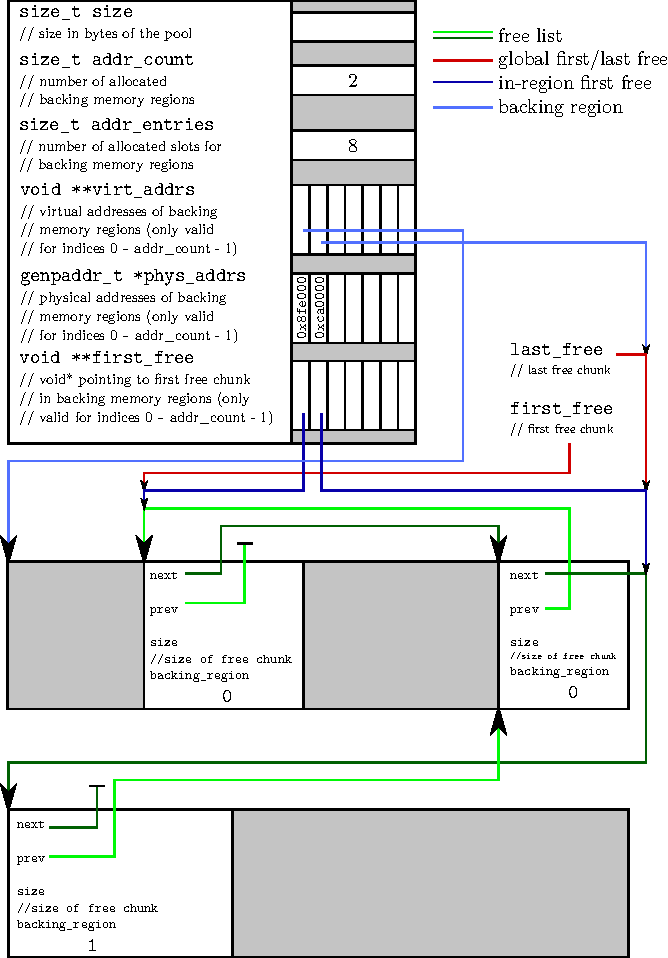
\includegraphics[width=.85\textwidth]{dma_pool_design.pdf}
\caption{DMA Buffer Pool Design}
\label{fig:dma_pool_design}
\end{figure}

\subsection{Design}

The pool memory is organized in regions which are allocated and mapped using
\linebreak\lstinline+frame_alloc+ and \lstinline+vspace_map_one_frame+
respectively. The virtual and physical addresses of each of these regions are
stored in the fields \lstinline+vaddr+ and \lstinline+paddr+ of
\linebreak\lstinline+struct dma_pool+ (c.f.~\autoref{fig:dma_pool_design}). The
\acs{dma} buffer pool uses a doubly linked free list for maintaining the free
chunks of the memory belonging to the pool.  A pointer to the first free chunk
of each backing region of the pool is stored in the pool metadata. Additionally
pointers to the first and last free chunk are stored.

When processing an allocation request, the free list is scanned from the front
for a sufficiently free chunk (first-free policy), which is returned in its
entirety if it is at most 512 bytes larger than the requested size or split
otherwise. If the chunk is split, the request is taken from the end of the
chunk and the beginning of the block is left in the free list. If the entire
chunk is returned, it is removed from the free list and the appropriate
metadata pointers (\lstinline+first_free+, \lstinline+last_free+, and
\lstinline+pool.first_free[backing_region]+) are updated, if necessary.

If there is no block large enough to satisfy the allocation request, the pool
is grown. This is done in steps of 8 megabytes at a time. Growing the pool
involves resizing the metadata arrays (\lstinline+virt_addrs+,
\lstinline+phys_addrs+, and \lstinline+first_free+) and allocating and mapping
memory for the new backing region.

Returning a block to the pool is similar: using the info in
\lstinline+pool.first_free+, a suitable point in the free list is found, and
the block is inserted into the free list. 

\subsection{Implementation}

\lstinline+ahci_dma_region_alloc+ searches through the free list linearly and
stops at the first free chunk that meets the condition {\tt request\_size <=
chunk\_size}. If no free chunk meets that condition \lstinline+grow_dma_pool+
is called to increase the pool size by eight megabytes and the free list
traversal continues with the new memory regions.  When a sufficiently large
free chunk is found, \lstinline+get_region+ is called.  That function checks if
the free chunk will be split or not (a chunk is split if the remaining free
chunk will be at least 512 bytes), allocates and constructs a
\lstinline+struct ahci_dma_region+ for the buffer that will be returned,
including computing the virtual and physical addresses of the buffer, and
shrinks the free chunk or removes it from the free list (according to the
chunk-splitting decision).

\lstinline+ahci_dma_pool_init+ calls \lstinline+grow_dma_pool+ with the
requested initial pool size rounded up to \lstinline+BASE_PAGE_SIZE+.

\lstinline+ahci_dma_region_free+ calls \lstinline+return_region+ on the passed
\lstinline+struct ahci_dma_region+. That function inserts the region into the
free list. Inserting the region into the free list can take different forms
according to the state of the free list before inserting the chunk.

After inserting the newly freed chunk into the free list,
\lstinline+return_region+ tries to merge the chunk with its predecessor and
successor in order to prevent excessive fragmentation of the buffer pool
memory.  After calling \lstinline+return_region+, the
\lstinline+struct ahci_dma_region+ is freed.

The last two functions (\lstinline+ahci_dma_region_copy_in+ and
\lstinline+ahci_dma_region_copy_out+) are implemented as
\lstinline+static inline+ and take a \lstinline+struct ahci_dma_region+, a
\lstinline+void*+ data
buffer, a \lstinline+genvaddr_t offset+ (into the \acs{dma} region), and a
\lstinline+size_t+ size. These functions just calculate the source (for
\lstinline+ahci_dma_region_copy_out+) or destination (for
\lstinline+ahci_dma_region_copy_in+) pointer for the memcpy and then copy the
data.

\newcommand{\issuecmd}{\lstinline+ahci_issue_command+\xspace}
\section[libahci Interface]{\libahci Interface}

\subsection[ahci\_issue\_command]{\issuecmd}

\issuecmd is the main function of libahci and takes a \lstinline+void*+ tag
with which the user can later match the command completed messages to his
issued commands, a \ac{fis} and \ac{fis} length, a boolean flag
\lstinline+is_write+ which indicates if \acs{dma} takes place to or from the
disk, and a \lstinline+struct vregion*+ data buffer and associated length.

\newcommand{\setupcmd}{\lstinline+ahci_setup_command+\xspace} First off
\issuecmd calls \setupcmd which allocates a command slot in the port's command
header. After that, \setupcmd allocates a command table for the new command
that has enough entries to accomodate $\lceil
data\_length\allowbreak/\allowbreak prd\_size\rceil$ \acp{prd}. Then \setupcmd
inserts the newly allocated command table into the reserved slot in the port's
command header and sets the bit to indicate the \acs{dma} direction (according
to \lstinline+is_write+) and also sets the \ac{fis} length in the command
header slot.  Finally, the \ac{fis} is copied into the newly allocated command
table and the \lstinline+int *command+ output parameter is assigned the command
slot number of the new command.

\newcommand{\addprs}{\lstinline+ahci_add_physical_regions+\xspace} After
completion of \setupcmd, \issuecmd saves the user's tag into the command slot
metadata and proceeds to call \addprs. This function takes the command slot
number (\lstinline+int commmand+) and a data buffer, partitions the data buffer
into physical regions and inserts those regions into the command slot indicated
by \lstinline+command+. The size of the physical regions is specified as at
most 4MB and must be an even byte count. However, due to hardware-related
problems when using physical regions larger than 128kB we artificially cap the
physical region size at 128kB. Memory addresses have to be word aligned.  If a
constant and predictable physical region size is desired, one can define
\lstinline+AHCI_FIXED_PR_SIZE+ and \lstinline+PR_SIZE+ to enforce a specific
size for physical regions.

Finally \issuecmd sets the issue command bit for the command slot in which the
new command is stored and calls the user continuation, if any.

\subsection{Command Completed Callback}

The command completed callback is called when the \ac{ahci} management daemon
receives a interrupt targeted to the \ac{ahci} port which is coupled with the
associated \lstinline+struct ahci_binding+. The command completed callback can
be adjusted by user code in order to post-process (cleanup, copy-out of read
data, etc.) a completed \ac{ahci} command.

The management command completed callback in \libahci (which is called from
ahcid when the port associated with the current libahci binding receives an
interrupt) reads the commmand issue register of the port and calls the
user-supplied command completed callback for each command slot which is marked
\lstinline+in_use+ in libahci but which has the corresponding bit in the
command issue register cleared.

The user-supplied command completed callback takes a \lstinline+void *tag+ as
its only argument; these tags are also saved in libahci, and should uniquely
identify their correpsonding \ac{ahci} command.

\newcommand{\ahciinit}{\lstinline+ahci_init+\xspace}
\subsection[ahci\_init]{\lstinline+ahci_init+}

\ahciinit is the first function a user of \libahci calls. \ahciinit initializes
the \lstinline+struct ahci_binding+ for the connection and if the connection to
\emph{ahcid} has not yet been established, tries to bind to \emph{ahcid}.  The
initalization of \libahci continues when the bind callback that was specified
in the call to \emph{ahcid} executes.

On the first call to \ahciinit, the bind callback sets up the function table
for the management binding and then calls \lstinline+ahci_mgmt_open_call__tx+
to request the port specified by the \lstinline+uint8_t port+ parameter of
\ahciinit from \emph{ahcid}. The initialization finishes when the ahci
management open callback executes.

On later \ahciinit calls \ahciinit updates the \emph{ahcid} binding to know
about the new \libahci connection and directly calls
\lstinline+ahci_mgmt_open_call__tx+.

The open callback checks if the open call succeeded, and if so, the memory
region containing the registers belonging to the requested port is mapped in
the address space in which \libahci executes. After that the receive \ac{fis}
area and the command list are set up, a copy of the \texttt{IDENTIFY} data is
fetched from \emph{ahcid}, the port is enabled (the \emph{command list running}
flag is set to one) and all port interrupts are enabled.

\subsection[ahci\_close]{\lstinline+ahci_close+}

The purpose of \lstinline+ahci_close+ is to release the port by calling the
close function of \emph{ahcid} (c.f.~\autoref{code:ahci_mgmt.if}). This needs
to be done, as otherwise \emph{ahcid} will return \verb+AHCI_ERR_+
\verb+PORT_BUSY+ on subsequent open calls for the same port.

\subsection[sata\_fis.h]{\lstinline+sata_fis.h+}

This header contains definitions dealing with \ac{sata}'s \ac{fis} that are
used for sending commands over \ac{ahci}. While the \ac{ata} command
specification defines what registers exist for each \ac{fis} type and how they
are used, the \ac{sata} specification defines the binary layout of these
registers.

While it might initially seem that a mackerel specification for these
structures would be sufficient, complexity introduced through optional \ac{ata}
features makes a custom API preferable. As an example, consider the layout of
28-bit and 48-bit \acp{lba}: for 28 bit \acp{lba}, the lower 24 bits are placed
in registers \verb+lba0+ through \verb+lba2+, while the upper 4 bits are placed
in the low bits of the \verb+device+ register. However, for 48-bit \ac{lba},
the \verb+device+ register is not used, and the upper 24 bits are placed in
register \verb+lba3+ through \verb+lba5+, which are separate from the lower 3
\verb+lba+ registers.

\section{Error Handling}

A mandatory part of an \ac{ahci} driver is to check if the \ac{hba} signals any
errors on command completion. \libahci does check the relevant registers, but
the only error handling implemented right now is to dump the registers
specifying the error and then aborting the domain that received the error.

In order to comply to the \ac{ahci} specification, the software stack (i.e.
\libahci) should attempt to recover. Errors signaled by one of the \verb+HBFS+,
\verb+HBDS+, \verb+IFS+ or \verb+TFES+ interrupts are fatal and will cause the
\ac{hba} to stop processing commmands. To recover from a fatal error, the port
needs to be restarted and any pending commands have to be re-issued to the
hardware or user level code has to be notified that these commands failed.

Errors signaled by the \verb+INFS+ or \verb+OFS+ interrupts are not fatal and
the \ac{hba} continues processing commands. In this case the software stack
does not have to take any action.
